\hypertarget{background}{%
\chapter{Background}\label{background}}

The relevant background we will need to acquaint ourselves with falls
into two halves: explaining the concept of a ``programming system'', and
explaining how the Three Properties tie together existing concepts in
programming. In Section~\ref{programming-systems-vs-languages}, we
define \emph{programming systems} in contrast to programming languages
and discuss why this is necessary. Subsequently, in
Section~\ref{examples-of-programming-systems}, we illustrate this with
landmark examples of programming systems from the past. Finally, in
Section~\ref{precursors-of-the-three-properties}, we survey the existing
patterns in programming that take us part of the way to the Three
Properties.

\hypertarget{programming-systems-vs-languages}{%
\section{Programming Systems vs
Languages}\label{programming-systems-vs-languages}}

Many forms of software have been developed to enable programming. The
classic form consists of a \emph{programming language}, a text editor to
enter source code, and a compiler to turn it into an executable program.
Instances of this form are differentiated by the syntax and semantics of
the language, along with the implementation techniques in the compiler
or runtime environment. Since the advent of graphical user interfaces
(GUIs), programming languages can be found embedded within graphical
environments that increasingly define how programmers work with the
language---for instance, by directly supporting debugging or
refactoring. Beyond this, the rise of GUIs also permits diverse visual
forms of programming, including visual languages and GUI-based end-user
programming tools.

The classic essay by Gabriel~\cite{PLrev} distinguishes the
\emph{languages} and \emph{systems} paradigms in programming research.
\emph{Languages} are formal mathematical models of syntax and semantics;
researchers might ask what an expression \emph{means} and include code
samples in papers. \emph{Systems,} in contrast, are running pieces of
software whose current state changes according to the effects of program
code. Researchers studying systems might be more concerned with what
code \emph{does} to a running system in a specific state instead of the
more abstract language properties.

The topic of this thesis, and many of the examples we will use to
illustrate concepts, rely on understanding this distinction and only
make sense within the systems paradigm. Therefore we shift our attention
from \emph{programming languages} to the more general notion of
``software that enables programming''---in other words,
\emph{programming systems}.

\begin{defn}[Programming System]
\label{def:programming-system}
A \emph{programming system} is an integrated and complete set of tools sufficient for creating, modifying, and executing programs. These will include notations for structuring programs and data, facilities for running and debugging programs, and interfaces for performing all of these tasks. Facilities for testing, analysis, packaging, or version control may also be present. Notations include programming languages and interfaces include text editors, but are not limited to these.
\end{defn}

A word about terminology: if we view languages in the sense of Gabriel's
``languages paradigm'', then it is a ``type error'' to include languages
in the above definition. Abstract mathematical models of syntax and
semantics are not the same as software. However, language
\emph{implementations} are software. We will use the term ``language''
to abbreviate ``language implementation'' since we have no use for the
other meaning in this dissertation.

With that said, our above notion of programming system covers classic
programming languages together with their editors, debuggers, compilers,
and other tools. Yet it is intentionally broad enough to \emph{also}
accommodate image-based programming environments like Smalltalk,
operating systems like Unix, and hypermedia authoring systems like
Hypercard, in addition to various other examples we will mention next.

\hypertarget{examples-of-programming-systems}{%
\section{Examples of Programming
Systems}\label{examples-of-programming-systems}}

We illustrate the notion of a programming system through a number of
example systems. We are not trying to exhaustively cover all possible
systems, but simply give an impression based on major examples.
Therefore, we draw them from three broad reference classes:

\begin{itemize}
\tightlist
\item
  Software ecosystems built around a text-based programming
  \emph{language}. They consist of a set of tools such as compilers,
  debuggers, and profilers. These tools may exist as separate
  command-line programs, or within an Integrated Development Environment
  (IDE).
\item
  Those that resemble an \emph{operating system} (OS) in that they
  structure the execution environment and encompass the resources of an
  entire machine (physical or virtual). They provide a common interface
  for communication, both between the user and the computer, and between
  programs themselves.
\item
  Programmable \emph{applications}, typically optimised for a specific
  domain, offering a limited degree of programmability which may be
  increased with newer versions.
\end{itemize}

\joel{
We will proceed to detail some systems under this grouping. This will provide an intuition for the notion of a programming system and establish a collection of go-to examples for the rest of the paper.}

\hypertarget{systems-based-around-languages}{%
\subsection{Systems Based Around
Languages}\label{systems-based-around-languages}}

Text-based programming languages sit within programming systems whose
boundaries are not explicitly defined. To speak of a programming system
we must include a language with, at minimum, an editor and a compiler or
interpreter. There is wiggle room in how we choose to circumscribe these
elements. Do we mean a specific compiler version? Do we include common
plugins or extensions? Still, we would expect these choices to have
enough of a common overlap that we can proceed with analysis without
worrying too much about the variations.

\paragraph{Java with the Eclipse ecosystem.}

The Java language~\cite{Java} alone does not form a programming system,
but it does if we consider it as embedded in an ecosystem of tools. A
minimalistic delineation would consist of a text editor to write Java
code and a command line compiler. A more realistic one is Java as
embedded in the Eclipse IDE~\cite{Eclipse}. The programming systems view
permits us to see whatever there may be beyond the textual code. In the
case of Eclipse, this includes the debugger, refactoring tools, testing
and modelling tools, GUI designers, and so on.

\paragraph{Haskell tools ecosystem.}

Haskell is another language-focused programming system. It is used
through the command-line \emph{GHC} compiler~\cite{GHC} and \emph{GHCi}
REPL, alongside a text editor that provides features like syntax
highlighting and auto-completion. Any editor that supports the Language
Server Protocol~\cite{LSP} will suffice to complete the programming
system.

Haskell is mathematically rooted and relies on mathematical intuition
for understanding many of its concepts. This background is also
reflected in the notations it uses. In addition to the concrete language
syntax for writing code, the ecosystem also uses an informal
mathematical notation for writing about Haskell (e.g.~in academic papers
or on the whiteboard). This provides an additional tool for manipulating
Haskell programs. Experiments on paper can provide a kind of rapid
feedback that other systems may provide through live programming.

\paragraph{From REPLs to Computational Notebooks.}

A different kind of developer ecosystem that evolved around a
programming language is the Jupyter notebook platform~\cite{Jupyter}. In
Jupyter, data scientists write scripts divided into notebook cells,
execute them interactively and see the resulting data and visualisations
directly in the notebook itself. This brings together the REPL, which
dates back to conversational implementations of Lisp in the 1960s, with
literate programming~\cite{LiterateProg} used in the late 1980s in
Mathematica 1.0~\cite{Mathematica}.

As a programming system representative of Computational
Notebooks~\cite{CompNotebooks}, Jupyter has a number of interesting
characteristics. The primary outcome of programming is the notebook
itself, rather than a separate application to be compiled and run. The
code lives in a document format, interleaved with other notations. Code
is written in small parts that are executed quickly, offering the user
more rapid feedback than in conventional programming. A notebook can be
seen as a trace of how the result has been obtained, yet one often
problematic feature of notebooks is that some allow the user to run code
blocks out-of-order. The code manipulates mutable state that exists in a
``kernel'' running in the background. Thus, retracing one's steps in a
notebook is more subtle than in, say, Common Lisp~\cite{CommonLisp},
where the \texttt{dribble} function would directly record the user's
session to a file.

\hypertarget{os-like-programming-systems}{%
\subsection{OS-Like Programming
Systems}\label{os-like-programming-systems}}

``OS-likes'' begin from the 1960s when it became possible to interact
one-on-one with a computer. At first, time-sharing systems enabled
interactive shared use of a computer via a teletype; smaller computers
such as the PDP-1 and PDP-8 provided similar direct interaction, while
1970s workstations such as the Alto and Lisp Machines added graphical
displays and mouse input. These \emph{OS-like} systems stand out as
having the totalising scope of \emph{operating systems}, whether or not
they are ordinarily seen as taking this role.

\paragraph{MacLisp and Interlisp.}

LISP 1.5~\cite{LISP15} arrived before the rise of interactive computers,
but the existence of an interpreter and the absence of declarations made
it natural to use Lisp interactively, with the first such
implementations appearing in the early 1960s. Two branches of the Lisp
family~\cite{LispEvolve}, MacLisp and the later Interlisp, embraced the
interactive ``conversational'' way of working, first through a teletype
and later using the screen and keyboard.

Both MacLisp and Interlisp adopted the idea of \emph{persistent address
space}. Both program code and program state were preserved when powering
off the system, and could be accessed and modified interactively as well
as programmatically using the \emph{same means}. Lisp Machines embraced
the idea that the machine runs continually and saves the state to disk
when needed. Today, this \emph{persistence}
(Definition~\ref{def:persistence}) is widely seen in cloud-based
services like Google Docs and online IDEs. Another idea pioneered in
MacLisp and Interlisp was the use of \emph{structure editors}. These let
programmers work with Lisp data structures not as sequences of
characters, but as nested lists. In Interlisp, the programmer would use
commands such as \texttt{*P} to print the current expression, or
\texttt{*(2\ (X\ Y))} to replace its second element with the argument
\texttt{(X\ Y)}. The PILOT system~\cite{Pilot} offered even more
sophisticated conversational features. For typographical errors and
other slips, it would offer an automatic fix for the user to
interactively accept, modifying the program in memory and resuming
execution. This is something that is only possible with Lisp's
\emph{naïve pokeability} (Definition~\ref{def:naive-pokeability}).

\paragraph{Smalltalk.}

Smalltalk appeared in the 1970s with a distinct ambition of providing
``dynamic media which can be used by human beings of all
ages''~\cite{PersonalDynMedia}. The authors saw computers as
\emph{meta-media} that could become a range of other media for
education, discourse, creative arts, simulation and other applications
not yet invented. Smalltalk was designed for single-user workstations
with a graphical display, and pioneered this display not just for
applications but also for programming itself. In Smalltalk 72, one wrote
code in the bottom half of the screen using a structure editor
controlled by a mouse, and menus to edit definitions. In Smalltalk-76
and later, this had switched to text editing embedded in a \emph{class
browser} for navigating through classes and their methods.

Similarly to Lisp systems, Smalltalk adopts the persistent address space
model of programming where data remains in memory, but based on
\emph{objects} and \emph{message passing} instead of \emph{lists}. Any
changes made to the system state by programming or execution are
preserved when the computer is turned off (this is \emph{persistence},
Definition~\ref{def:persistence}). Lastly, the fact that much of the
Smalltalk environment is implemented in itself makes it possible to
extensively modify the system from within.

We include Lisp and Smalltalk in the OS-likes because they function as
operating systems in many ways. On specialised machines, like the Xerox
Alto and Lisp machines, the user started their machine directly in the
Lisp or Smalltalk environment and was able to do everything they needed
from \emph{within} the system. Nowadays, however, this experience is
associated with Unix and its descendants on a vast range of commodity
machines.

\paragraph{Unix.}

Unix fits Definition~\ref{def:programming-system} and illustrates the
fact that many aspects of programming systems are shaped by their
intended target audience. Built for computer hackers~\cite{Hackers}, its
abstractions and interface are close to the machine. Although
historically linked to the C language, Unix developed a
language-agnostic set of abstractions that make it possible to use
multiple programming languages in a single system. While everything is
an object in Smalltalk, the ontology of Unix consists of files, memory,
executable programs, and running processes. Note the explicit ``stage''
distinction here: Unix distinguishes between volatile \emph{memory}
structures, which are lost when the system is shut down, and
non-volatile \emph{disk} structures that are preserved. This distinction
between types of memory is considered, by Lisp and Smalltalk, to be an
implementation detail to be abstracted over by their persistent address
space. Still, this did not prevent the Unix ontology from supporting a
pluralistic ecosystem of different languages and tools. Thus Unix is
distinguished as a \emph{meta-}programming system, supporting the
creation and interaction of different programming systems within it. We
will go into more detail on these points in
Section~\ref{the-unix-paradigm}.

\paragraph{Early and modern Web.}

The Web evolved~\cite{DotCom} from a system for sharing and organising
information to a \emph{programming system}. Today, it consists of a wide
range of server-side programming tools, JavaScript and languages that
compile to it, notations like HTML and CSS, and the sophisticated
developer tools included in browsers. As a programming system, the
``modern 2020s web'' is reasonably distinct from the ``early 1990s
web''. In the early web, JavaScript code was distributed in a form that
made it easy to copy and re-use existing scripts, which led to
enthusiastic adoption by non-experts---recalling the birth of
microcomputers like Commodore 64 with BASIC a decade earlier.

In the ``modern web'', multiple programming languages treat JavaScript
as a compilation target, and JavaScript is also used as a language on
the server-side. This web is no longer simple enough to encourage
copy-and-paste remixing of code from different sites. However, as we
observed in Section~\ref{web-pages-web-apps-and-browsers} it does come
with advanced developer tools providing functionality resembling that of
Lisp and Smalltalk. The Document Object Model (DOM) almost resembles the
tree/graph model of Smalltalk and Lisp images, lacking the key
persistence property (Definition~\ref{def:persistence}). Such a
limitation can be surpassed by efforts like
Webstrates~\cite{Webstrates}, which synchronise the DOM between the
server and clients. Thus if a client changes an element, this can be
mirrored on the server side and saved as the ground truth of the web
page.

\paragraph{COLAs.}

The one system that directly influenced our work is the Combined Object
Lambda Architecture or COLA~\cite{COLAs}: a small, expressive starting
system designed for open evolution by its user. It is described as a
mutually self-implementing pair of abstractions: a structural object
model (the ``Object'' in the acronym) and a behavioural Lisp-like
language (the ``Lambda''). COLA aims for maximal openness to
modification, down to the basic semantics of object messaging and Lisp
expressions.

The two remarkable features we see in the COLA idea are
\emph{self-sustainability} and a hint at \emph{notational freedom},
which we will say more about in
Section~\ref{precursors-of-the-three-properties}. COLA inherits
self-sustainability from the Smalltalk tradition and attempts to amplify
it. This provides for what the authors refer to as \emph{internal
evolution} as a means for implementing \emph{mood-specific languages:}

\begin{quote}
Applying {[}internal evolution{]} locally provides scoped,
domain-specific languages in which to express arbitrarily small parts of
an application (these might be better called \emph{mood-specific}
languages). Implementing new syntax and semantics should be (and is) as
simple as defining a new function or macro in a traditional language.
\end{quote}

An example of a mood-specific language is the one reported
in~\cite[p.\ 4]{Steps08} for concisely specifying how TCP packets should
be processed. The report also notes:

\begin{quote}
The header formats are parsed from the diagrams in the original
specification documents, converting ``ascii art'' into code to
manipulate the packet headers.
\end{quote}

This machine interpretation of ASCII art diagrams is another example of
a mood-specific language, and we see this as the extreme end of what
they are capable of. The ability for a programmer to express arbitrarily
small parts of an application in a form they deem suitable is, in its
fully \emph{general} form, what we call Notational Freedom. With such a
capability, code could be synthesised from \emph{real} tabular diagrams
of packet headers, not just those rendered with ASCII characters.

\hypertarget{application-focused-systems}{%
\subsection{Application-Focused
Systems}\label{application-focused-systems}}

The previously discussed programming systems were either universal, not
focusing on any particular kind of application, or targeted at broad
fields, such as Artificial Intelligence and symbolic data manipulation
in Lisp's case. In contrast, the following examples focus on narrower
application domains. Many support programming based on rich interactions
with specialised visual and textual notations.

\paragraph{Spreadsheets.}

The first spreadsheets became available in 1979 in
VisiCalc~\cite{VisiCalc, VisiCalc2} and helped analysts perform budget
calculations. As programming systems, spreadsheets are notable for their
two-dimensional grid substrate and their model of automatic
re-evaluation. The programmability of spreadsheets developed over time,
acquiring features that made them into powerful programming systems in a
way VisiCalc was not. A major step was the 1993 inclusion of
\emph{macros} in Excel, later further extended with \emph{Visual Basic
for Applications} and more recently with \emph{lambda functions.}

\paragraph{HyperCard.}

While spreadsheets were designed to solve problems in a specific
application area, HyperCard~\cite{HyperCard} was designed around a
particular application format. Programs are ``stacks of cards''
containing multimedia components and controls such as buttons. These
controls can be programmed with pre-defined operations like ``navigate
to another card'', or via the HyperTalk scripting language for anything
more sophisticated.

As a programming system, HyperCard is interesting for a couple of
reasons. It effectively combines visual and textual notation. Programs
appear the same way during editing as they do during execution. Most
notably, HyperCard supports gradual progression from the ``user'' role
to ``developer'': a user may first use stacks, then go on to edit the
visual aspects or choose pre-defined logic until, eventually, they learn
to program in HyperTalk.

\paragraph{Graphical languages.}

Efforts to support programming without relying on textual code are
``languages'' in a more metaphorical sense. In the ``boxes-and-wires''
style of LabView~\cite{LabView} programs are made out of graphical
structures. There is also the Programming-By-Example~\cite{YWIMC} subset
in which a general program is automatically generated by the user
supplying sample behaviours and hints.

\hypertarget{precursors-of-the-three-properties}{%
\section{Precursors of the Three
Properties}\label{precursors-of-the-three-properties}}

In the next chapter, we will go on to develop the Three Properties in
detail. However, they do not leap out of a vacuum, but are rather
developments of concepts that already exist in programming. Here, we
will give a glossary of these existing concepts. In short:

\begin{itemize}
\tightlist
\item
  Self-Sustainability is foreshadowed by self-hosting compilers and
  reflection.
\item
  Notational Freedom generalises domain-specific languages and polyglot
  programming.
\item
  Explicit Structure already exists in the form of data structures and
  various editors.
\end{itemize}

\hypertarget{precursors-of-self-sustainability}{%
\subsection{Precursors of
Self-Sustainability}\label{precursors-of-self-sustainability}}

\paragraph{Self-hosting.}

This describes a compiler that can compile its own source code into a
functionally identical compiler program. We can then change the language
understood by the compiler by changing the source code, compiling it
with the current version, and discarding this version in favour of the
new one. We can then rewrite the compiler's source code to make use of
the new language feature. In this way, a programming language can be
evolved using itself and we can call the language ``self-hosting'' (as a
proxy for its compiler.)

\paragraph{Bootstrapping.}

This is the process of getting a language into a self-hosting
state~\cite{Bootfrom0}. Suppose we design a novel language
\emph{NovLang} and we are happy to use C++ to build its compiler.
Bootstrapping it consists of the following steps:

\begin{enumerate}
\def\labelenumi{\arabic{enumi}.}
\tightlist
\item
  We write a NovLang compiler in NovLang, but we cannot run it yet.
\item
  We translate this by hand to C++ and build a temporary NovLang
  compiler.
\item
  We run this to compile the NovLang source code from step 1.
\item
  We obtain a runnable compiler for NovLang, which was written in
  NovLang and is now self-hosting.
\item
  We can now discard the C++ code.
\end{enumerate}

\paragraph{Meta-circular.}

This describes an interpreter that is written in its own
language~\cite{Metac}. This was first introduced in Lisp, in which one
can write Lisp code to walk nodes in a data structure and treat them as
Lisp expressions. If such code was compiled, it would result in an
ordinary Lisp interpreter. Alternatively, if we feed such code into an
existing Lisp interpreter, this new inner interpreter is now
meta-circular. We could change the code to add a new language feature,
in which case the inner interpreter would understand this slightly
improved language. However, this approach does not scale, as each
improvement would nest a further interpreter within the previous ones,
multiplying the overhead to impractical levels.

\paragraph{Reflection.}

This is the capacity for a system to display, explain or affect its own
computational behaviour during run time~\cite{CompRefl}. It is sometimes
explained with the word ``aboutness'': an ordinary program is ``about''
its domain (say, calculations), while a reflective program is also
``about'' its own computation. One test of this is the ability to make
the tacit explicit~\cite{ProcRefl}: entities that are normally implicit
and unaddressable (such as the stack frame or variable binding
environment) can be made so by an explicit command to reflect. An
ordinary meta-circular interpreter cannot name its outer interpreter's
data structures, but a reflective one can (and may be able to change how
its outer interpreter works, and thus how it itself works.) This is
developed exhaustively for Lisp-like languages in~\cite{ProcRefl}. While
reflection originates as a property of languages, the Self
environment~\cite{Self} provides an example in an interactive context.
Any object on screen can call up an ``outliner'' object with a
description of its prototype, private state and methods. This outliner
is an object and can have the same operation applied to it.

\paragraph{Conclusion.}

These concepts---self-hosting, bootstrapping, meta-circularity, and
reflection---seem related but it is not obvious how. We interpret all of
these as different manifestations of self-sustainability in special
contexts, such as compilers or interpreters. In Chapter~\ref{analysis}
we will make this more precise by delving into the differences between
compilers, interpreters, and interactive programming systems.

\hypertarget{precursors-of-notational-freedom}{%
\subsection{Precursors of Notational
Freedom}\label{precursors-of-notational-freedom}}

\paragraph{\URTFJ.}

This is a widespread maxim in programming~\cite{RightTool}. The ideal
conditions capturing the spirit of this idea are as follows.

\paragraph{Subjective Preference.}

What is ``right'' is subjectively determined by the programmer, even on
a whim. Ordinarily, when proposing a change to a language (e.g.~Python),
every user of the language is forced to confront the change, which
invites debate about what is ``right'' for everyone. This could be
sidestepped if each programmer could use what is right, for their own
context, without this being forced on others. This is meant even in a
collaborative context: ideally, each collaborator may use their chosen
tool and a common infrastructure or format allows their efforts to
cohere.

\paragraph{Metaphorical Tool.}

The ``tool'' might be an entire programming system or language, a design
approach, or simply a notation in which to express a component.

\paragraph{Range of Scopes.}

The ``job'' can be large (an entire project), small (a single
expression) or anything in-between.

Even though these are ideal conditions that we do not inhabit, being
aware of them lets us get a sense of how applicable this principle is
and opens us to any low-hanging fruit in this area. We will now review
the limited extent to which we can apply the principle in our actual
environment of programming.

\paragraph{Polyglot Programming.}

This is the practice of using multiple languages in a single
project~\cite{Polyglot}. Modules implemented in different languages need
to share data and invoke each other's functions, for which there are
several approaches:

\begin{itemize}
\tightlist
\item
  If the modules are separate programs, standard inter-process
  communication mechanisms like interchange file formats (JSON, XML),
  socket protocols, and Remote Procedure Calls are available.
\item
  Polyglot programming \emph{within} a shared process address space is
  trickier; the classic approach is to have different languages (e.g.~C,
  Pascal) compile to a common \emph{object file} format understood by
  the linker. This method is restricted to compile-time; for runtime
  sharing, languages use Foreign Function Interfaces (FFIs). This
  practice has been critiqued by Kell~\cite{KellMMM} who advocates the
  use of ``integration domains'' instead.
\item
  Polyglot programming within a single \emph{file} is rare and
  restricted to fixed combinations. Perl and JavaScript support regexes
  written with a local syntax. HTML files include not only HTML but also
  JavaScript and CSS. C\# supports Language INtegrated Queries (LINQ)
  which are a C\# syntax adaptation of SQL queries. Unlike the freedom
  to choose any combination of existing languages for an entire project,
  these instances only permit use of a pre-approved set decided by the
  language designers.
\end{itemize}

\paragraph{Domain-Specific Languages (DSLs).}

These go beyond Polyglot Programming by encouraging \emph{custom}
languages designed by the programmer for their problem domain. Where
Polyglot Programming is about making the best use of \emph{existing}
languages designed by someone else, DSLs come closer to a \emph{freedom}
to use what one subjectively determines to be the best tool for one's
job. JetBrains' MPS~\cite{MPS} is an interactive programming system that
encourages DSLs. ``Reader Macros'' in Lisp allow a programmer to use
custom syntax for parts of the code. The COLA design~\cite{COLAs}
supports ``mood-specific languages'' intended to span a range of scopes
down to individual expressions, and the related OMeta~\cite{OMeta}
project is a platform for custom DSLs. The Eco editor~\cite{Eco} also
supports mood-specific languages and even more general notations.

\paragraph{Conclusion.}

``\URTFJ'' is the basic intuition behind Notational Freedom. In
practice, we see a restricted version: use the right \emph{pre-existing}
tool for the job, as long as the job is no smaller than a single file.
Occasionally, a pre-approved set of different languages are available
within a single file. In the rare cases that support the use of custom
``tools'' within a file, we risk being restricted to \emph{languages}
rather than general \emph{notations.} Only MPS and Eco, as far as we are
aware, go ``all the way'' in this regard. We will continue this
discussion in more detail in Chapter~\ref{analysis}.

\hypertarget{precursors-of-explicit-structure}{%
\subsection{Precursors of Explicit
Structure}\label{precursors-of-explicit-structure}}

\hypertarget{representation}{%
\subsubsection{Representation}\label{representation}}

\paragraph{Structure.}

This is the relation of parts to wholes. An entire data structure is
made up of smaller parts which reference each other. From a machine's
point of view, a data structure is a graph of memory blocks connected by
numerical pointers. For humans, it is a graph of dictionaries with named
entries, some of which point at other dictionaries. Both of these models
can be visualised as boxes with arrows.

\paragraph{Binary files.}

These are \emph{compacted} data structures. Unlike data structures in
memory, which can be sparsely spread across large regions and
intermingled with each other, a binary file will often contain the parts
densely packed together without any unrelated data. If not, the binary
file serves as an uncompacted ``image'' of a region or regions of
memory.

\paragraph{Syntax.}

In programming, this refers to the ``look and feel'' of a language's
textual source code. Formally, syntax is the set of rules defining legal
and illegal symbol sequences. This idea can be metaphorically extended
to non-sequential structures. For example, we can think of C
\texttt{struct} definitions as setting out the valid ``shape'' of the
parts of a data structure. The same applies to binary file formats.

\paragraph{Quantitative Syntax.}

This is a term introduced by~\cite[p.\ 13]{Infra} for the pattern of
prefixing a block with its length and using numerical pointers to link
structures. A simple example is the Pascal String which begins with a
length byte and continues for that many characters.

\paragraph{Qualitative Syntax.}

This, in contrast to Quantitative Syntax, relies on special delimiters.
For example, the C String begins right away with its characters, relying
on a null byte to show up at some point and signal the end.

\hypertarget{formats}{%
\subsubsection{Formats}\label{formats}}

\paragraph{Text files, a.k.a. Strings.}

These are lists of plain text characters. In programming, they are often
containers for machine-readable structures as an alternative to binary
files. Like the latter, they compact the structure, but in a way subject
to the constraints of plain text and qualitative syntax. In practice,
the structure in question is usually a tree, in which case the string is
built as an \emph{in-order} traversal. This means that special
qualitative syntax (usually the matched bracket characters \texttt{(},
\texttt{{[}}, \texttt{\{}, or \texttt{\textless{}}) is employed
\emph{around} substrings to encode the structure.

\paragraph{Parsing and serialising.}

These convert between strings and structures. Parsing \emph{recovers}
structure implicit in a string, while serialising spins out the
structure into a string.

\paragraph{Format error.}

This is a part of a data structure that violates a decidable expectation
of its consumer. For example, a syntactically valid file containing
program source code might violate static typing rules or use a name that
was not declared. Undecidable ``semantic'' rules like prohibiting
division by zero are excluded from this term (see
Figure~\ref{fig:format-errors}).

\paragraph{Syntax error.}

This is a special case of format error where part of a text string
violates a grammatical expectation of its consumer.

\begin{figure}
\centering

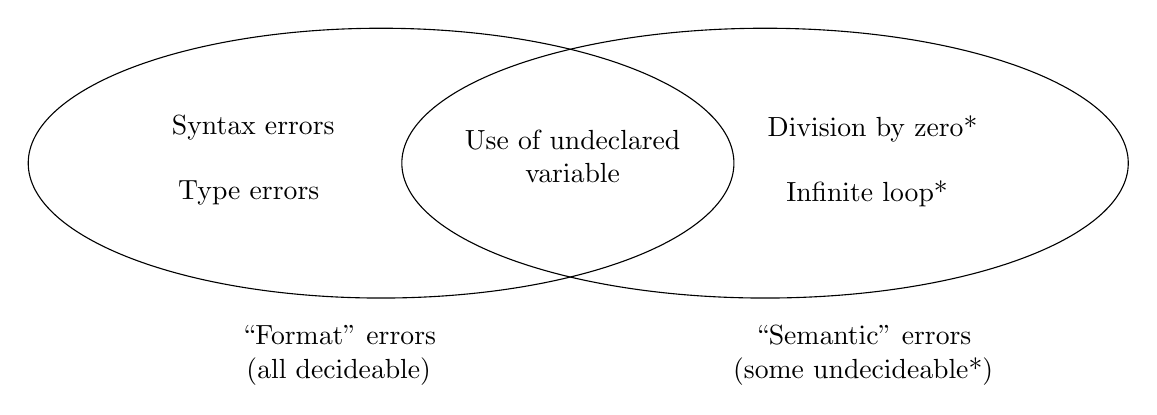
\begin{tikzpicture}[x=0.75pt,y=0.75pt,yscale=-1,xscale=1]
%uncomment if require: \path (0,300); %set diagram left start at 0, and has height of 300

%Shape: Ellipse [id:dp5326335354678456] 
\draw   (210,85) .. controls (210,49.1) and (288.35,20) .. (385,20) .. controls (481.65,20) and (560,49.1) .. (560,85) .. controls (560,120.9) and (481.65,150) .. (385,150) .. controls (288.35,150) and (210,120.9) .. (210,85) -- cycle ;
%Shape: Ellipse [id:dp904564307478004] 
\draw   (30,85) .. controls (30,49.1) and (106.11,20) .. (200,20) .. controls (293.89,20) and (370,49.1) .. (370,85) .. controls (370,120.9) and (293.89,150) .. (200,150) .. controls (106.11,150) and (30,120.9) .. (30,85) -- cycle ;

% Text Node
\draw (98,61) node [anchor=north west][inner sep=0.75pt]   [align=left] {Syntax errors};
% Text Node
\draw (351,162) node [anchor=north west][inner sep=0.75pt]   [align=left] {\begin{minipage}[lt]{120pt}\setlength\topsep{0pt}
\begin{center}
“Semantic" errors\\(some undecideable*)
\end{center}

\end{minipage}};
% Text Node
\draw (125,162) node [anchor=north west][inner sep=0.75pt]   [align=left] {\begin{minipage}[lt]{80pt}\setlength\topsep{0pt}
\begin{center}
“Format" errors\\(all decideable)
\end{center}

\end{minipage}};
% Text Node
\draw (101,92) node [anchor=north west][inner sep=0.75pt]   [align=left] {Type errors};
% Text Node
\draw (231,68) node [anchor=north west][inner sep=0.75pt]   [align=left] {\begin{minipage}[lt]{90pt}\setlength\topsep{0pt}
\begin{center}
Use of undeclared\\variable
\end{center}

\end{minipage}};
% Text Node
\draw (385,61) node [anchor=north west][inner sep=0.75pt]   [align=left] {Division by zero*};
% Text Node
\draw (394,92) node [anchor=north west][inner sep=0.75pt]   [align=left] {Infinite loop*};


\end{tikzpicture}

\caption{Format errors include syntax errors, type errors and some ``semantic'' errors as long as they are decideable.}
\label{fig:format-errors}
\end{figure}

\hypertarget{editors}{%
\subsubsection{Editors}\label{editors}}

\paragraph{Editors.}

These are programs for creating various data structures in the form of
files. Editors for 3D models, vector graphics, raster images, audio, and
video understand the file formats and strive to save only valid files.
It is usually not possible to even \emph{express} a structure in the
editor that contains a format error. Such cases are exceptional: for
example, a 3D scene might open without errors in another 3D editor, but
cause errors in a game engine according to the latter's additional
requirements---perhaps it expects specific objects in the scene named
\texttt{Player}, \texttt{Exit}, and so on. Nevertheless, for most
editors and most use cases, the consumer-side validity rules are in
harmony with the producer-side rules.

\paragraph{Text Editors.}

These are a type of editor for plain text files. However, they are
widely used to write code in programming languages, which have extra
syntax rules beyond the plain text format. Unlike most editors, text
editors \emph{can} save files that are invalid from the perspective of
their consumers under realistic use-cases. These syntax errors are then
discovered at the point of consumption.

\paragraph{Conclusion.}

The basic intuition behind Explicit Structure is the \emph{directness}
experienced in creation and programming. Almost every data structure in
computing has an editor with which one can manipulate the structure
directly, and when programming we can act as if data structures have
named parts that we can simply reference. This directness is interrupted
by the standalone exception of text editors (on the creation side) and
strings with machine-readable\footnote{We are unconcerned with strings
  that contain natural language simply to be echoed out to the user
  (e.g.~error messages). However, our ideas about Explicit Structure may
  be applicable to cases where software must parse and interpret natural
  language too.} implicit content (on the programming side).
